\section{Metodologia de investigacion}

Para la metodología de investigación que se llevó a cabo en este proyecto, se consideraron los niveles de madurez tecnológica (TRLs) del Ministerio de Ciencia, Tecnología e Innovación de Colombia, que son un sistema de medición sistemático para evaluar la madurez de una tecnología específica y compararla con otras tecnologías \cite{minciencias2018TRL}. De acuerdo con estos niveles, ilustrados en la figura \ref{fig:trl}, el proyecto se situó entre los niveles TRL 3 y TRL 4, lo que indicó que se encontraba en una fase de validación conceptual y evaluación inicial del prototipo en un entorno controlado, correspondiente a la población y al alcance planteado.

\begin{figure}[H]
    \centering
    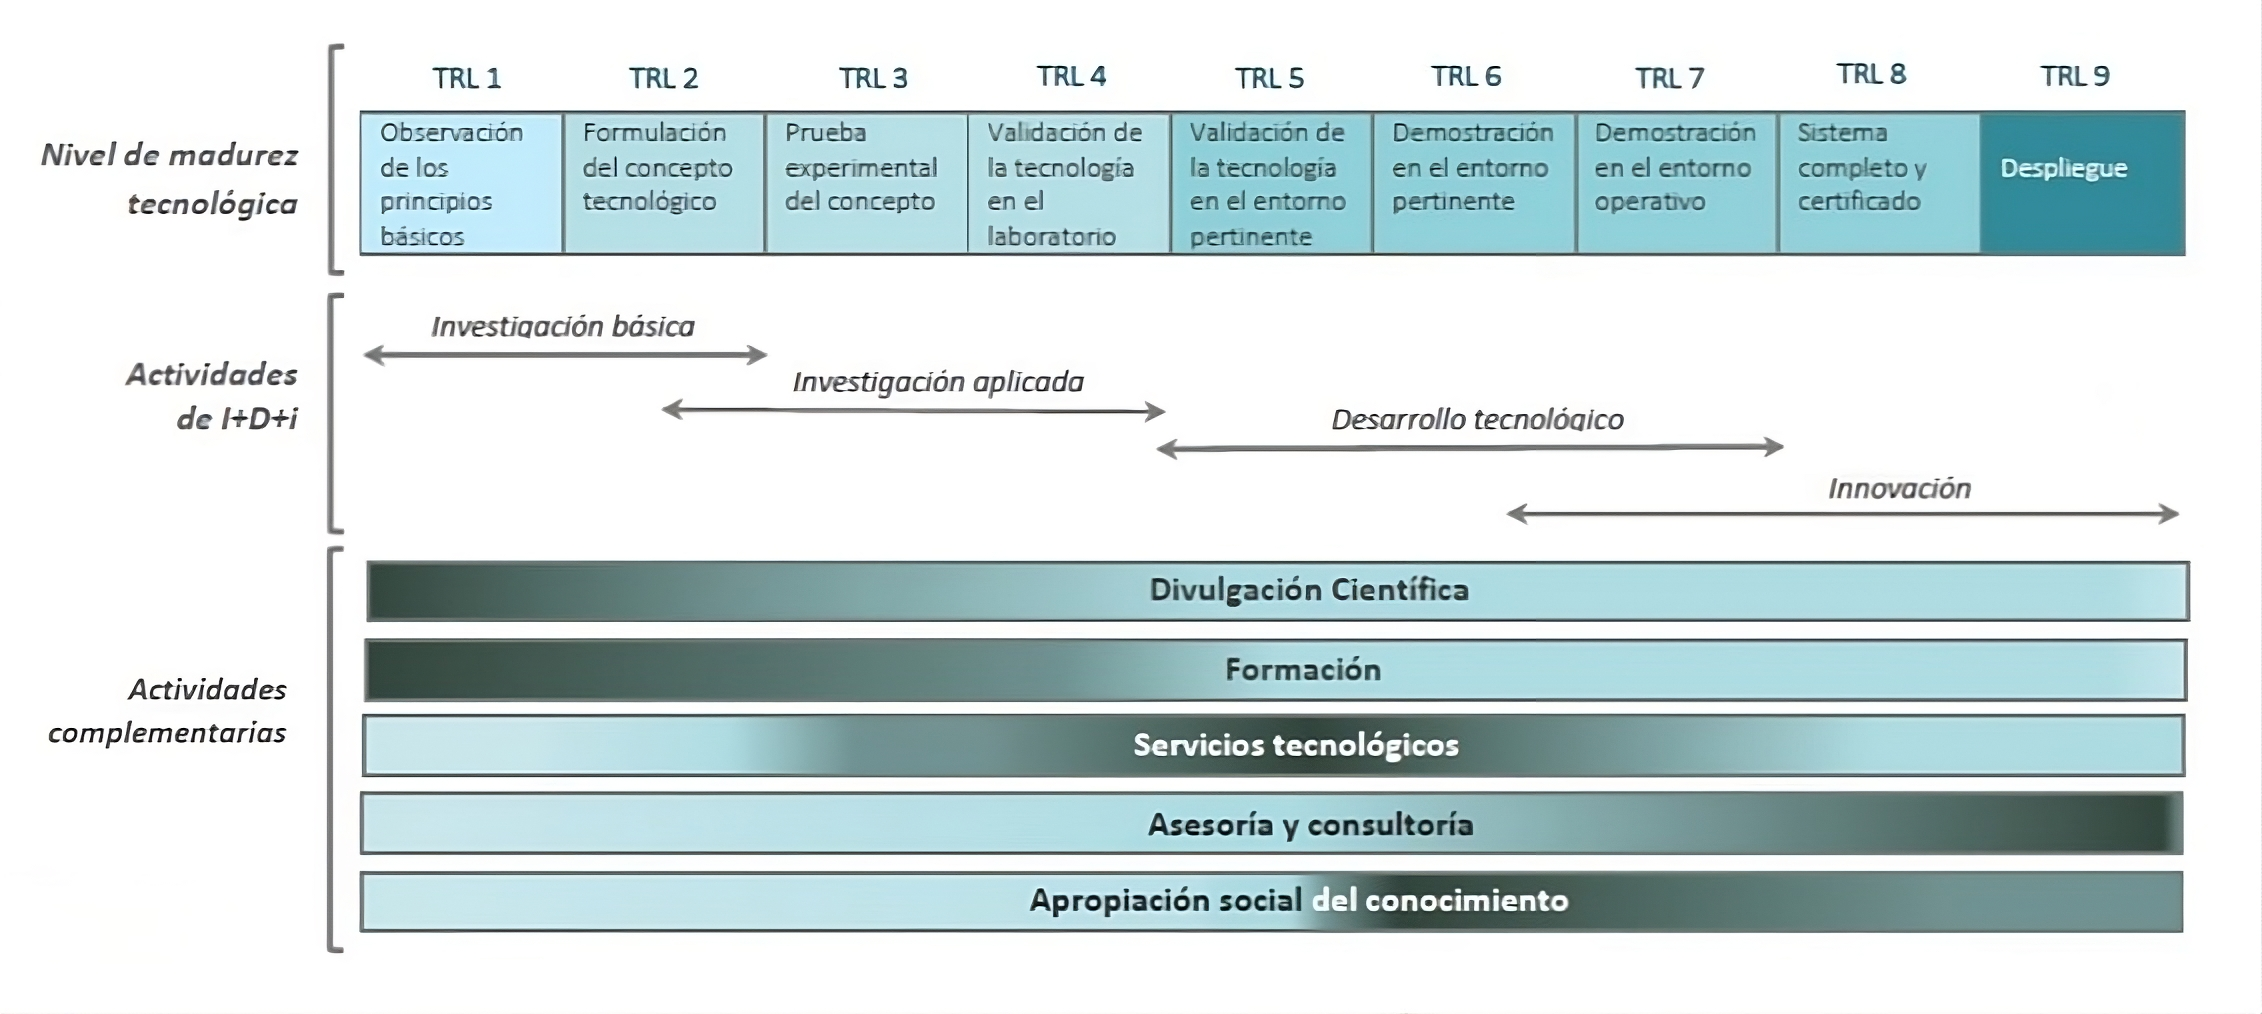
\includegraphics[width=\textwidth]{Figuras/trl.png}
    \caption{Niveles de TLR}
    \label{fig:trl}
\end{figure}

Este enfoque metadológico permitió aplicar los conocimientos adquiridos a lo largo de la formación profesional, con el fin de impulsar tanto el desarrollo como la validación de tecnologías en un contexto práctico y pertinente.
\\ \\
Teniendo en cuenta esta metodología de investigación, se siguió una secuencia de etapas orientadas a garantizar un proceso eficiente.  En primer lugar, se realizó una búsqueda bibliográfica para recopilar información relevante sobre el desarrollo de las habilidades seleccionadas, así como los métodos educativos y tecnologías de enseñanza disponibles. Posteriormente, se desarrolló la fase de diseño y construcción del software, utilizando diversas tecnologías web y herramientas de desarrollo. Una vez finalizada esta etapa, se procedió a la recolección de datos y evaluación mediante encuestas y actividades de desempeño, con el fín de analizar la efectividad del software en el desarrollo de habilidades blandas. Finalmente, se examinaron los datos obtenidos para elaborar conclusiones y formular recomendciones para ajustes o posibles mejoras futuras en la plataforma.